\documentclass[10pt,a4paper]{report}
%\usepackage[latin1]{inputenc}
\usepackage{blindtext}
\usepackage{multicol}
\usepackage[utf8]{inputenc}
\usepackage{amsmath}
\makeatletter
\newcommand\xleftrightarrow[2][]{%
  \ext@arrow 9999{\longleftrightarrowfill@}{#1}{#2}}
\newcommand\longleftrightarrowfill@{%
  \arrowfill@\leftarrow\relbar\rightarrow}
\makeatother
\usepackage{amsfonts}
\usepackage{amssymb}
\usepackage{graphicx}
\usepackage{multicol}
\usepackage{tabularx}
\usepackage{tikz}
\usepackage{hyperref}
\hypersetup{
colorlinks=true,
linkcolor=blue,
filecolor=blue,
citecolor = black,
urlcolor=blue,
}
\usetikzlibrary{arrows,shapes,automata,petri,positioning,calc}
\usepackage{hyperref}
\usepackage{tikz}
\usetikzlibrary{matrix,calc}
\newcommand{\myvec}[1]{\ensuremath{\begin{pmatrix}#1\end{pmatrix}}}
\usepackage[margin=0.5in]{geometry}
\providecommand{\norm}[1]{\left\lVert#1\right\rVert}
%\newcommand{\myvec}[1]{\ensuremath{\begin{pmatrix}#1\end{pmatrix}}}
\let\vec\mathbf
\newcommand{\mydet}[1]{\ensuremath{\begin{vmatrix}#1\end{vmatrix}}}
%\newcommand{\myvec}[1]{\ensuremath{\begin{pmatrix}#1\end{pmatrix}}}
%\let\vec\mathbf
\providecommand{\mtx}[1]{\mathbf{#1}}
\newenvironment{Figure}
  {\par\medskip\noindent\minipage{\linewidth}}
  {\endminipage\par\medskip}
\begin{document}
%--------------------logo figure-------------------------%
\begin{figure*}[!tbp]
  \centering
  \begin{minipage}[b]{0.4\textwidth}
   
\includegraphics[scale=0.5]{iithlogo.png} 
  \end{minipage}
  \hfill
  \vspace{5mm}\begin{minipage}[b]{0.4\textwidth}
\raggedleft 
\includegraphics[scale=0.5]{nrc.jpeg} 
  \end{minipage}\vspace{0.2cm}
\end{figure*}
%--------------------name & rollno-----------------------
\raggedright 
\begin{center}
\Large \textbf{Circle Assignment}\hspace{2.5cm} %
\end{center}
\begin{center}
\hspace{0.5cm}
\textbf{Name}:\hspace{2mm}Rupa Sai Sreshta Vallabhaneni\hspace{1cm}
\date{25-September-2022}
\end{center}
%\begin{center}
%\end{center}  
%\normalsize \textbf{Roll No.} :\hspace{1mm} FWC22047\vspace{1cm}
%\begin{multicols}{2}
%\begin{tableofcontents}
%\begin{tableofcontents}
\begin{multicols}{2}
\section*{Problem Statement}
From the point A(0,3) on the circle $x^2+4x+(y-3)^2=0$. A chord AB is drawn and extended to a point M.Such that AM=2AB. Find the equation of locus of M.
\section*{Construction}
\hspace{0.25cm}
\begin{tabular}{|c|c|c|}
	\hline
	\textbf{Symbol}&\textbf{Value}&\textbf{Description}\\
	%\hline
	%$\vec{U_1}$ & $\begin{pmatrix}0 \\ 0 \\ \end{pmatrix}$ & center of given circle\\
	\hline
    $\vec{A}$&$\myvec{0 \\ 3}$&Point on given circle\\
	\hline
	$\vec{M}$&$\myvec{h \\ k}$ & Point outside circle\\
	 \hline
	 $\vec{B}$ & $\myvec{\frac{h}{2} \\ \frac{k+3}{2}}$& Mid point of A and M\\

	 %Circle equation &  $x^2+4x+(y+3)^2=0$ & Equation of circle \\
	 \hline
	 $\vec{r_1}$ & 2 & Radius of given circle\\
	 \hline
	 $\vec{C}$ & $\myvec{-2 \\ 3}$ & Center of given circle\\
	 \hline
%	 \hline
%	$\begin{pmatrix}a & b \\ \end{pmatrix}$ & $\begin{pmatrix}1 & 2 \\ \end{pmatrix}$ & point on circle \\ \hline
\end{tabular}
%\hspace{2cm}\\
\vspace{0.5cm}\\
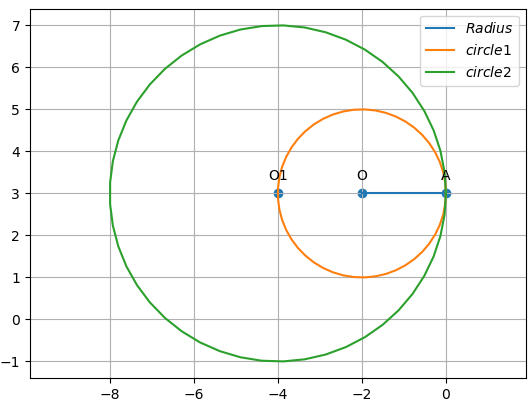
\includegraphics[scale=0.4]{circle2.png}
\begin{center}
Figure of construction
\end{center} 
You can download the python code for generating above circle from the below link
\vspace{0.25cm}\\
\boxed{Github link: \href{https://github.com/RupaSaiSreshta/FWC}{https://github.com/RupaSaiSreshta/FWC}}
\section*{Solution}
Given $\vec{A}$=$\myvec{0 \\ 3}$
\vspace{0.25cm}\\
AM=2AB
\vspace{0.25cm}\\
From this condition B is the midpoint of A and M.
\\
The given circle equation is 
\begin{align}
\vec{x}^{\top}\vec{V}\vec{x}+2\vec{u}^{\top}\vec{x}+f=0
\end{align}
\vspace{0.25cm}\\
$\vec{V}$=$\vec{ \begin{pmatrix}1 & 0 \\ 0 & 1 \end{pmatrix}}$, 
\vspace{0.25cm}\\
$\vec{u}$=$\vec{ \begin{pmatrix}2 \\ -3 \end{pmatrix}}$, 
\vspace{0.25cm}\\
f = 9.

%\vspace{0.25cm}\\
%Given circle equation is  $x^2+4x+(y+3)^2=0$
%\vspace{0.25cm}\\
%This can be written as $x^2+y^2+4x-6y+9=0$
%\vspace{0.25cm}\\
%With the given circle equation $x^2+y^2+4x-6y+9=0$, we can find the center C and radius r1 of the circle.
%\vspace{0.25cm}\\
Center of the circle 
\begin{align} 
\vec{C} &= \myvec{-2 \\ 3} 
\end{align}
Radius of the circle
\begin{align}
{\vec{r_1}=2}
\end{align}
Let us assume %\begin{align}
\vspace{0.25cm}
\\$\vec{M}$ =$\myvec{h \\ k}$
%\end{align}
\vspace{0.25cm}\\
As B is the midpoint of A and M
\vspace{0.25cm}\\
Then 
\vspace{0.25cm}\\
%\begin{align}
$\vec{B}$ =$\myvec{\frac{h}{2} \vspace{0.15cm}\\ \frac{k+3}{2}}$
%\end{align}
\vspace{0.25cm}\\
Consider 
\vspace{0.25cm}\\
$\vec{x}$=$\myvec{\frac{h}{2} \vspace{0.15cm}\\ \frac{k+3}{2}}$
\vspace{0.25cm}\\
Now substitute $\vec{x}$ , $\vec{V}$ , $\vec{u}$ , f in Equation 1\vspace{0.25cm}\\
%\vspace{3.5cm}\\
\begin{align}
\begin{pmatrix} 
\frac{h}{2} & \frac{k+3}{2} 
\end{pmatrix} 
\begin{pmatrix}
1 & 0\\ 0 & 1 \\
\end{pmatrix}
\begin{pmatrix}
\frac{h}{2} \\ \frac{k+3}{2} 
\end{pmatrix}+2
\begin{pmatrix}
-2 & 3
\end{pmatrix}
\begin{pmatrix}
\frac{h}{2} \\ \frac{k+3}{2} 
\end{pmatrix}+9=0
\end{align}
%\hspace{1cm}
By solving 
\vspace{0.25cm}\\
We get
\vspace{0.25cm}\\
$\vec{ \begin{pmatrix}h & k \end{pmatrix}}$
$\vec{ \begin{pmatrix}1 & 0 \\ 0 & 1 \end{pmatrix}}$
$\vec{ \begin{pmatrix}h \\ k \end{pmatrix}}$+2
$\vec{ \begin{pmatrix}4 & -3 \end{pmatrix}}$
$\vec{ \begin{pmatrix}h \\ k \end{pmatrix}}$+9=0
\vspace{0.25cm}\\
Now write this equation in terms of x and y
\vspace{0.25cm}\\
Then
\vspace{0.25cm}\\
$\vec{ \begin{pmatrix}x \\ y \end{pmatrix}}$
$\vec{ \begin{pmatrix}1 & 0 \\ 0 & 1 \end{pmatrix}}$
$\vec{ \begin{pmatrix}x & y \end{pmatrix}}$+2
$\vec{ \begin{pmatrix}4 & -3 \end{pmatrix}}$
$\vec{ \begin{pmatrix}x \\ y \end{pmatrix}}$+9=0
\\
The locus equation of M is
\begin{align}
\boxed {x^2+y^2+8x-6y+9=0}
\end{align}
%  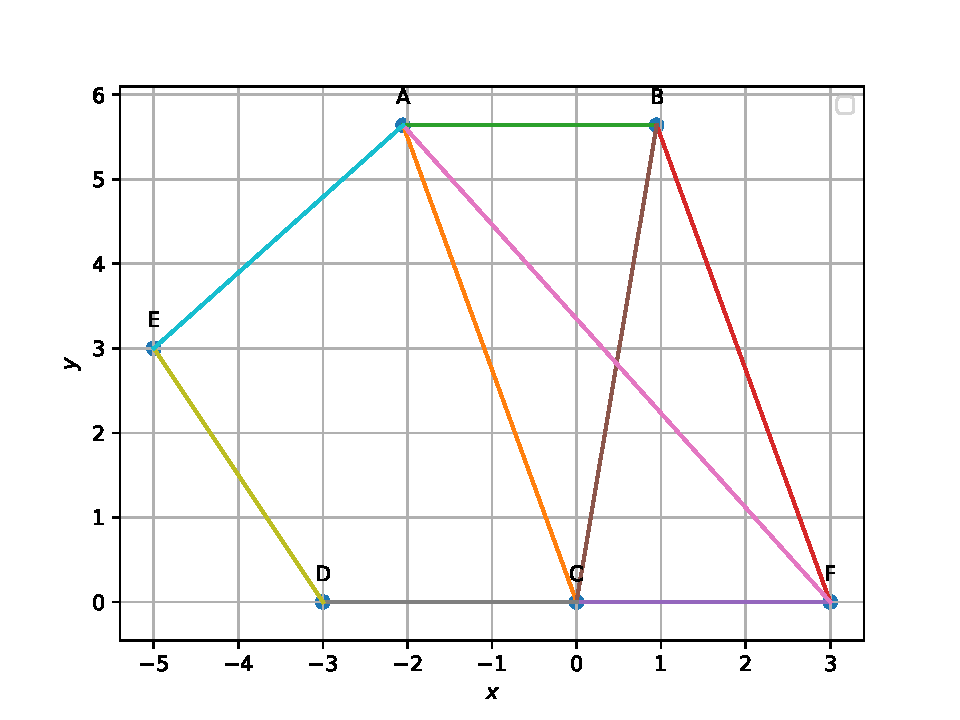
\includegraphics[scale=0.5]{/home/srinath/Documents/matrix.pdf} 
\end{multicols}
\end{document}